\documentclass[10pt]{article}

\def\Type{LessonDJ}
\def\TypeNum{Workshop Week 13} %Lesson #
\def\TypeTitle{Random Variables, PDFs, CDFs, Expected Value and Variance } %Lesson Title
\def\Semester{Fall 2021} %Not Used 
\def\Course{MATH 1190}%Course number and name
\def\Targets{   \target{P1}, \target{P2} }

\usepackage{preambleDJ} 

%%%%%%%%%%%% BEGIN DOCUMENT %%%%%%%%%%%%%%%
%%%%%%%%%%%% BEGIN DOCUMENT %%%%%%%%%%%%%%%
%%%%%%%%%%%% BEGIN DOCUMENT %%%%%%%%%%%%%%%
%%%%%%%%%%%% BEGIN DOCUMENT %%%%%%%%%%%%%%%
%%%%%%%%%%%% BEGIN DOCUMENT %%%%%%%%%%%%%%%

\begin{document}
\pagestyle{otherpages}
\thispagestyle{firstpage}


\vs{.6}
\section{Discrete vs Continuous}
Determine whether each random variable is discrete or continuous. Briefly explain your reasoning.

\enumA{
        \item The exact amount of rainfall (in inches) recorded at a weather station during a 24-hour period.
        \item The number of customers who enter a store between 10:00 AM and 11:00 AM.
        \item The weight (in grams) of a randomly selected apple from a large orchard.
        \item The number of heads obtained when a fair coin is flipped 10 times.
        \item The exact height (in centimeters) of a randomly selected student in the class.
}


\newpage
\section{Probability Density and Cumulative Distribution Function}
Let \( T \) be a continuous random variable with the probability density function
    \[
    p(t) = 
    \begin{cases} 
    c\cdot t^6 & -1 \leq t \leq 1, \\
    0 & \text{otherwise}.
    \end{cases}
    \]
    \enumA{
        \item Determine the value of the constant \( c \) that makes \( p(t) \) a valid PDF.
        \item Find the CDF (cumulative distribution function) \( F(t) \).
        \item Use $F(t)$ to compute the probability that \( T \) is greater than 0.6, i.e. $P(T>0.6)$. You will want to use technology to calculate the final step.
        \item Find the  \( m \) such that \( P(T \leq m) = 0.5 \). The value  $m$ is called the {\em median}.
}
\newpage

\section{Expected Value and Variance (Discrete)}
Recall that in the discrete case the expected value (or mean) and the variance are defined as
\[
\mu=E[X]=\sum_{i=1}^nx_i \cdot p(x_i)
\]
\[
Var(X)= \sum_{i=1}^n (x_i-\mu)^2\cdot p(x_i)=  \left( \sum_{i=1}^n x_i^2\cdot p(x_i)  \right) -\mu^2
\]
The histogram below represents the PDF of a random variable $X$. \\
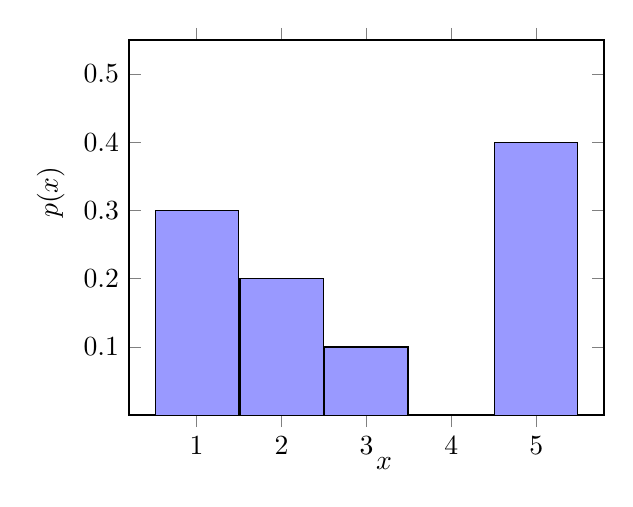
\begin{tikzpicture}
    \begin{axis}[
        ybar, % Specifies vertical bars
        bar shift=0,
        ymin=0, % Ensures bars start from zero
        xtick={1,2,3,4,5}, % Places x-axis ticks at data points
	%xticklabels={,,,,,,}, % Custom x-axis labels
	xticklabels={$1$,$2$,$3$,$4$,$5$},
	ytick       = {0.1,0.2,0.3,0.4,0.5},
            %yticklabels =  {$1/16$,$2/16$,$3/16$, $4/16$},
        enlarge x limits={0.2}, % Adjusts spacing between bars and axis limits
            y label style={anchor=south west},
            ylabel={$p(x)$},
                        xlabel = {$x$},
		x label style={anchor=west},
		 ymin = 0, ymax = .55,
        bar width=30pt, % Adjusts the width of the bars
                    width = 3in, height=2.5in,
          %          enlarge x limits={1.2},
      	axis line style={thick, ->},
    ]
% \addplot[fill=blue!40] coordinates {(1,0)  (2,0)  (3,0) (4,0) (5,0)};
  \addplot[fill=blue!40] coordinates {(1,0.3)  (2,0.2)  (3,0.1) (4,0) (5,0.4)};
    \end{axis}
\end{tikzpicture}

\enumA{
    \item Compute the expected value of $X$, $E(X)$.
    \item Compute the variance of $X$, $Var(X)$.
    \item Sketch a histogram that would have the same mean as $x$ but would have a {\em higher} variance. Remember that the total probability must always be $1$.\\
\begin{tikzpicture}
    \begin{axis}[
        ybar, % Specifies vertical bars
        bar shift=0,
        ymin=0, % Ensures bars start from zero
        xtick={1,2,3,4,5}, % Places x-axis ticks at data points
	%xticklabels={,,,,,,}, % Custom x-axis labels
	xticklabels={$1$,$2$,$3$,$4$,$5$},
	ytick       = {0.1,0.2,0.3,0.4,0.5},
            %yticklabels =  {$1/16$,$2/16$,$3/16$, $4/16$},
        enlarge x limits={0.2}, % Adjusts spacing between bars and axis limits
            y label style={anchor=south west},
            ylabel={$p(x)$},
                        xlabel = {$x$},
		x label style={anchor=west},
		 ymin = 0, ymax = .55,
        bar width=30pt, % Adjusts the width of the bars
                    width = 3in, height=2.5in,
          %          enlarge x limits={1.2},
      	axis line style={thick, ->},
    ]
 \addplot[fill=blue!40] coordinates {(1,0)  (2,0)  (3,0) (4,0) (5,0)};
  %\addplot[fill=blue!40] coordinates {(1,0.3)  (2,0.2)  (3,0.1) (4,0) (5,0.4)};
    \end{axis}
\end{tikzpicture}

}



\newpage
\section{Expected Value and Variance (Continuous)}
Recall that in the continuous case the expected value (or mean) and the variance are defined as
\[
\mu=E[X]=\int_a^b x \cdot p(x) dx
\]
\[
Var(X)=\int_a^b(x-\mu)^2 \cdot p(x) dx=\left( \int_a^b x^2 \cdot p(x) dx \right) -\mu^2
\]
\mpageT{.5}{.5}{
Let $X$ be a continuous random variable with probability density function $p(x)$.
$$
  p(x)=\begin{cases} 
    c (1-x^2) & -1 \leq x \leq 1, \\
    0 & \text{otherwise}.
    \end{cases}
$$
}{\centering
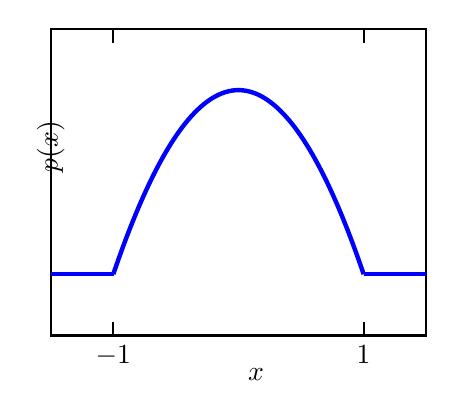
\begin{tikzpicture}
\begin{axis}[
	x label style={anchor=west},
xlabel={$x$},
xtick       = {-1,1},
xticklabels = {$-1$,$1$},
xticklabel style={anchor=north},
y label style={anchor=west},
ylabel={$p(x)$},
ytick=\empty,
%ytick       = {1/30},
yticklabels = {},
samples     = 320,
xmin =-1.5, xmax = 1.5,
ymin = -.25, ymax = 1.,
axis line style = {  thick, -},
every major tick/.append style={  thick, black, major tick length=5pt},
width=2.5in
]
\addplot[ultra thick, blue, domain=-1:1] {3/4*(1-x^2)};
\addplot[ultra thick, blue, domain=-1.5:-1] {0};
\addplot[ultra thick, blue, domain=1:1.5] {0};
\end{axis}
\end{tikzpicture}
%
%
%
}
\enumA{
    \item Find the value of $c$ that will ensure that this is a probability density function.
    \item Compute the expected value $E[X]$;
    \item Compute the variance $Var(X)$;
}

\newpage


\section{Probability Density Function}\label{sec}
Consider the continuous random variable $X$ with the following probability density function p(x) and it's graph:\\
\mpageT{.5}{.5}{\centering
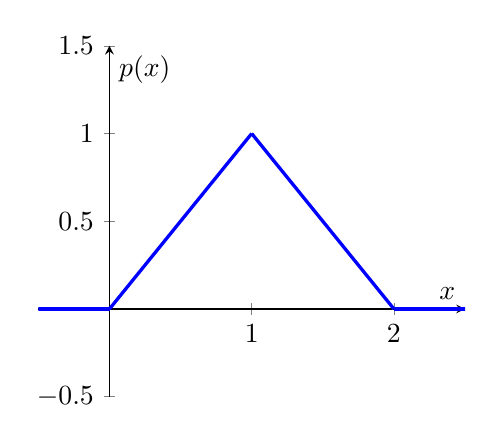
\begin{tikzpicture}
\begin{axis}[
    axis lines = middle,
    xlabel = $x$,
    ylabel = $p(x)$,
    xmin = -0.5, xmax = 2.5,
    ymin = -0.5, ymax = 1.5,
    samples = 200,
    domain = -0.5:2.5,
    width=7cm,
]
% f(x)=x on [0,1]
\addplot[very thick, blue, domain=0:1] {x};
% f(x)=2-x on [1,2]
\addplot[very thick, blue, domain=1:2] {2 - x};
% f(x)=0 elsewhere: left part
\addplot[very thick, blue, domain=-0.5:0] {0};
% right part
\addplot[very thick, blue, domain=2:2.5] {0};
\end{axis}
\end{tikzpicture}
}{
\[
p(x) =
\begin{cases}
0 & x < 0, \\[6pt]
x & 0 \le x \le 1, \\[6pt]
2 - x & 1 \le x \le 2, \\[6pt]
0 & x > 2.
\end{cases}
\]
}
\enumA{
\item Check that $p(x)$ is truly a probability density function, which means that you have to check the two defining properties.
\item Compute $P(X \leq 0)$, $P(X \geq 0.5)$, $P(X \leq 1)$, $\ds P(X=1/3)$;
\item Find an interval $[0,b]$ where $P(0\leq X \leq b)=1/8$  
}



%
%\newpage 
%\section{Piecewise Cumulative Distribution Function} 
%Consider the continuous random variable from section \# \ref{sec}, which had the probability density function:
%\\ 
%\mpageT{.5}{.5}{\centering
%\begin{tikzpicture}
%\begin{axis}[
%    axis lines = middle,
%    xlabel = $x$,
%    ylabel = $p(x)$,
%    xmin = -0.5, xmax = 2.5,
%    ymin = -0.5, ymax = 1.5,
%    samples = 200,
%    domain = -0.5:2.5,
%    width=7cm,
%]
%% f(x)=x on [0,1]
%\addplot[very thick, blue, domain=0:1] {x};
%% f(x)=2-x on [1,2]
%\addplot[very thick, blue, domain=1:2] {2 - x};
%% f(x)=0 elsewhere: left part
%\addplot[very thick, blue, domain=-0.5:0] {0};
%% right part
%\addplot[very thick, blue, domain=2:2.5] {0};
%\end{axis}
%\end{tikzpicture}
%}{
%\[
%p(x) =
%\begin{cases}
%0 & x < 0, \\[6pt]
%x & 0 \le x \le 1, \\[6pt]
%2 - x & 1 \le x \le 2, \\[6pt]
%0 & x > 2.
%\end{cases}
%\]
%}
%
%\enumA{
%    \item  Find the corresponding cumulative distribution function, $F(x)$ using steps a), b) and c) below Since $p(x)$ is a piecewise function, $F(x)$ will also be piecewise.
%   \[
%F(x) =
%\begin{cases}
%0 & x < 0, \\[6pt]
%F_1(x) & 0 \le x \le 1, \\[6pt]
%F_2(x) & 1 \le x \le 2, \\[6pt]
%1 & x > 2.
%\end{cases} 
%     \]
%    \enum{
%    \item Find the cumulative distribution function over the interval $0\leq x\leq 1$. Let's call this $F_1(x)$
%    \item Find the cumulative distribution function over the interval $1\leq x\leq 2$. Let's call this $F_2(x)$
%    \item Check two things: Is $F_1(1)=F_2(1)$? Is $F_2(2)=1$? If one/both are not true, you probably forgot to add something to the function $F_2(x)$.
%    }
%    \item Now graph this cumulative distribution function;
%    \item Use the cumulative distribution function to find the probability of $P(X \leq 1)$ and $P(X \in [0,1.5])$
%    \item  Use the cumulative distribution function to find an interval $[c,1]$ where $P(c\leq X\leq 1)=1/8$.
%}
%
%\newpage
%\section{More Piecewise Cumulative Distribution Function}
%Let \( X \) be a continuous random variable with the probability density function
%    \[
%    p(x) = 
%    \begin{cases} 
%    c(5 - x) &0 \leq x \leq 5, \\
%    c(x+5) &-5\leq x\leq0,
%    \\
%    0 & \text{otherwise}.
%    \end{cases}
%    \]
%\begin{enumerate}
%        \item Find the support of \( X \).
%        \item Determine the value of the constant \( c \) that makes \( p(x) \) a valid PDF.
%        \item Compute \( P(1 < X < 3) \).
%        \item Find the cumulative distribution function \( C(x) \) for \( -5 \leq x \leq 5 \) (You need to consider 2 different integrals for some situation).
%\end{enumerate}

\end{document}